\documentclass[12pt]{extarticle}

\usepackage[]{cite}
\usepackage{cmap}
\usepackage[T2A]{fontenc}
\usepackage[utf8]{inputenc}
\usepackage[english, russian]{babel}

\usepackage{tikz}
\usetikzlibrary{matrix}

% latin bold lower
\newcommand{\ba}{\mathbf{a}} 
\newcommand{\bb}{\mathbf{b}}
\newcommand{\bc}{\mathbf{c}} 
\newcommand{\be}{\mathbf{e}} 
\newcommand{\bh}{\mathbf{h}} 
\newcommand{\bp}{\mathbf{p}} 
\newcommand{\bq}{\mathbf{q}}
\newcommand{\bt}{\mathbf{t}} 
\newcommand{\bs}{\mathbf{s}} 
\newcommand{\bu}{\mathbf{u}} 
\newcommand{\bv}{\mathbf{v}} 
\newcommand{\bw}{\mathbf{w}} 
\newcommand{\bx}{\mathbf{x}} 
\newcommand{\by}{\mathbf{y}} 
\newcommand{\bz}{\mathbf{z}} 

% latin bold upper
\newcommand{\bA}{\mathbf{A}} 
\newcommand{\bB}{\mathbf{B}} 
\newcommand{\bC}{\mathbf{C}} 
\newcommand{\bD}{\mathbf{D}} 
\newcommand{\bE}{\mathbf{E}}
\newcommand{\bF}{\mathbf{F}}
\newcommand{\bH}{\mathbf{H}}
\newcommand{\bI}{\mathbf{I}} 
\newcommand{\bJ}{\mathbf{J}}
\newcommand{\bM}{\mathbf{M}} 
\newcommand{\bP}{\mathbf{P}}
\newcommand{\bQ}{\mathbf{Q}}
\newcommand{\bR}{\mathbf{R}}
\newcommand{\bS}{\mathbf{S}}
\newcommand{\bT}{\mathbf{T}} 
\newcommand{\bU}{\mathbf{U}} 
\newcommand{\bV}{\mathbf{V}} 
\newcommand{\bW}{\mathbf{W}} 
\newcommand{\bX}{\mathbf{X}} 
\newcommand{\bY}{\mathbf{Y}} 
\newcommand{\bZ}{\mathbf{Z}} 

% \usepackage{jmlda}
\newcommand{\hdir}{.}
\usepackage{amsmath, amsfonts,amssymb,mathrsfs}
\usepackage{graphicx}
\usepackage{minted}
\usepackage{hyperref}
\usepackage{mathtools}
\usepackage{tocloft}
\usepackage[linesnumbered,boxed]{algorithm2e}
% \usepackage{algorithm}
% \usepackage{algpseudocode}
% \usepackage[usenames]{color}
% \usepackage{colortbl}
\usepackage{setspace}
\doublespacing

\usepackage{graphicx, epsfig}
\usepackage{subfig}
\usepackage{color}

\usepackage{wrapfig}
\usepackage{float}
\usepackage{subfloat}
\usepackage{caption}
\usepackage{multirow}



\newtheorem{theorem}{Теорема}
\newtheorem{lemma}[theorem]{Лемма}
\newtheorem{definition}{Определение}
\newtheorem{remark}{Замечание}
\newenvironment{Proof} % имя окружения
    {\par\noindent{\bf Доказательство.}} % команды для \begin
    {\hfill$\scriptstyle\blacksquare$} % команды для \end

\DeclareMathOperator*{\argmax}{arg\,max}
\DeclareMathOperator*{\argmin}{arg\,min}
\newcommand{\Domain}{\mathcal{D}}
\newcommand{\supp}{\mathrm{supp}}
\newcommand{\diag}{\mathrm{diag}}
\newcommand{\bfw}{\mathbf{w}}
\newcommand{\bfv}{\mathbf{v}}
\newcommand{\bfx}{\mathbf{x}}
\newcommand{\bfz}{\mathbf{z}}
\newcommand{\bfX}{\mathbf{X}}
\newcommand{\bfy}{\mathbf{y}}
\newcommand{\bfb}{\mathbf{b}}
\newcommand{\bbr}{\mathbb{R}}
\newcommand{\bsigma}{\boldsymbol\Sigma}
\newcommand{\expectation}{\mathbb{E}}
\newcommand{\ceil}[1]{\lceil #1 \rceil}

\def\BibAuthor#1{\ruseng{\textit{#1}}}
\def\BibTitle#1{\ruseng{\textrm{#1}}}
\def\BibJournal#1{\ruseng{\textrm{#1}}{\textsl{#1}}}
\def\BibUrl#1{{\small\url{#1}}}
\def\BibHttp#1{{\small\url{http://#1}}}
\def\BibFtp#1{{\small\url{ftp://#1}}}
\def\BibDoi#1{doi:~{\small\url{http://dx.doi.org/#1}}}
\def\typeBibItem{\small\sloppy}


\textheight=22cm % высота текста
\textwidth=16cm % ширина текста
\oddsidemargin=0pt % отступ от левого края
\topmargin=-1.5cm % отступ от верхнего края
\parindent=24pt % абзацный отступ
\parskip=5pt % интервал между абзацами
\tolerance=2000 % терпимость к "жидким" строкам
\flushbottom % выравнивание высоты страниц

\begin{document}
\thispagestyle{empty}
\begin{center}
    \sc
        «Московский физико-технический институт \rm{(национальный исследовательский университет)}»\\
        Физтех-школа прикладной математики и информатики\\
        Кафедра <<Интеллектуальные системы>>
        %\\        при Вычислительном центре им. А. А. Дородницына РАН
        \\[35mm]
    \rm\large
        Курдюкова Антонина Дмитриевна\\[10mm]
    \bf\Large
		Снижение размерности фазового пространства в задачах канонического корреляционного анализа\\[10mm]
    \rm\normalsize
        03.03.01 -- Прикладные математика и физика\\[10mm]
    \sc
        Выпускная квалификационная работа бакалавра\\[10mm]
\end{center}
\hfill\parbox{85mm}{
    \begin{flushleft}
    \bf
        Научный руководитель:\\
    \rm
        д.ф.-м.н. Стрижов Вадим Викторович\\[3.9cm]
    \end{flushleft}
}
\begin{center}
    Москва\\
    2022
\end{center}

\newpage
\tableofcontents
\newpage

\begin{abstract}
Данная работа посвящена задаче снижения размерности фазового пространства методами канонического корреляционного~анализа. Исследуется связь между методом канонического корреляционного анализа и методом сходящихся перекрестных отображений Сугихары. Вид прогностических моделей представляется в виде условия принадлежности двух аттракторов к общей динамической системе. Аттракторы восстанавливаются в исходном и целевом фазовых пространствах. В работе рассмотрены метод проекций на латентные структуры, метод канонического кореляционного анализа, их нелинейные модификации, метод сходящихс] перекрестных отображений, seq2seq, Neural ODE. Сформулирован вариант теоремы о вложениях Такенса для проверки удовлетворенгия методов прогноза условиям Сугихары. Решается прикладная задача в восстановления траектории движения руки человека по сигналу акселерометра. Рассматривается видеоряд ходьбы человека с акселерометром на руке.
\\
\bigskip
\noindent

\textbf{Ключевые слова}: \emph {снижение размерности, фазовое пространство, аттрактор, метод сходящихся перекрестных отображений, теорема Такенса о вложениях}
\end{abstract}
\newpage

%данные поля заполняются редакцией журнала
% \doi{10.21469/22233792}
% \receivedRus{01.01.2017}
% \receivedEng{January 01, 2017}

% \maketitle

% \cftchapterprecistoc




\section{Введение}



% \addcontentsline{toc}{section}{\protect\numberline{}Введение}


Решается задача прогнозирования сигналов походки человека. Такие сигналы обладают сложной структурой. Под сложной структурой понимаются зависимости и изменяющийся период. Рассматриваются два связанных фазовых пространства. Одно из них является исходным, другое - целевым. Например, фазовое пространство сигналов акселерометра и гироскопа одного мобильного устройства; пространства сигналов двух акселерометров в правой и левой руке человека; пространство траектории движения руки, восстановленной по видеоряду движения человека, и пространство сигнала акселерометра на этой руке.

 Целью работы является построение более простой модели, работающей не хуже уже существующих моделей прогнозирования временных рядов.

Для улучшения качества прогноза, а также для упрощения прогностической модели предлагается учесть зависимости между временными рядами, а также перейти в пространство меньшей размерности. Снижение размерности позволяет учитывать внутреннее низкоразмерное проедставление временных рядов в прогностической модели. 

Для определения наличия связи между временными рядами используется метод сходящегося перекрестного отображения (convergent cross mapping, CCM) \cite{sugihara1990nonlinear, sugihara2012detecting}. Метод CCM проверяет, насколько близки точки фазового пространства временного ряда $s_1$, соответствующие ближайшим соседям ряда $s_2$.Под близостью понимается существование взаимно однозначного соответствия, которое отображает окрестность фазовой траектории $s_1$ в окрестность фазовой траектории $s_2$.

Для снижения размерности траекторного пространства используются метод проекций в латентное пространство (partial least squares PLS) \cite{geladi1988notes, hoskuldsson1988pls}, его нелинейная модификация \cite{yaushev}, seq2seq[..], NeuralODE[..]. Снижение размерности позволяет сделать прогностическую модель более устойчивой, изучить связь между главными компонентами временных рядов, а также найти траекторное подпространство, в котором удастся обнаружить связь между временными рядами.


В работе исследуется связь между методами корреляционного анализа и методом сходящегося перекрестного отображения. Требуется построить прогностическую модель, связывающую метод сходящегогся перекрестного отображения и методы канонического корреляционного анализа.
Для ССМ нет способа выбора собственного подпространства, в котором аппроксимируется многообразие компакта и работает прогностическая модель. На текущий момент выбор собственного пространства осуществляется перебором по главным компонентам, например в \cite{usmanova}. Работа Исаченко [..] по PLS дает возможность обобщить методы выбора подпространства с PLS на CCM.

\begin{definition}
Динамическая система -- множество элементов, для которого задана функциональная зависимость между временем и положением в фазовом пространстве каждого элемента системы.
\end{definition}
Динамическая система представляет собой такую математическую модель некоего объекта, процесса или явления, в которой пренебрегают <<флуктуациями и всеми другими статистическими явлениям>>.
\begin{definition}
Многообразие -- хаусдорфово топологическое пространство со счётной базой, каждая точка которого обладает окрестностью, гомеоморфной евклидову пространству $\bbr^n$
\end{definition}


\section{Постановка задачи}
Дан временной ряд $s_1 = \{s_i^1 \}_{i=1}^{N_1} $. Значения временного ряда заданы в моменты времени $1, \dots, N_1$. Требуется построить прогноз ряда на следующие $m$ значений $N_1+1, \dots, N_1+m$. 

При построении прогностической модели $\mathcal{F}$ нужно учесть влияние ряда $s_2~=~\{ s_i^2\}_{i=1}^{N_2}$ на ряд $s_1$. Значения ряда $s_2$ в моменты времени $N_1+1, \dots, N_1+m$ известны, то есть $N_2 > N_1 + m$.

Для построения прогноза ряда $s_1$ на один шаг по времени вперед будем учитывать $L$ предыдущих значений этого ряда и все предшествующие текущему моменту времени значения ряда $s_2$. Тогда прогностическая модель имеет вид:
\begin{equation}
    \widehat{s}\,_{t+1}^1 = \mathcal{F}(\widehat{\mathbf{w}}, s_{t}^1, \dots, s_{t-L+1}^1, s_1^2, \dots, s_t^2),
    \label{eq:F}
\end{equation}
    \[\widehat{\mathbf{w}} = \argmin_{\mathbf{w}}\,L(\mathbf{w}, s_1, \widehat{s_1}),\]
где $L$ ~--- функция потерь.



\section{Теоретическая часть}
    Пусть $s_1 = \{s_i^1\}_{i=1}^{N_1}$ и $s_2 = \{s_i^2 \}_{i=1}^{N_2}$ ~--- заданные временные ряды. Опишем, как строится фазовое пространство $\mathbf{X}$ временного ряда. Строится ганкелева матрица для ряда $s_1$:
     \[ \mathbf{H_1} = \begin{bmatrix}
                        s_1 & \dots & s_{n_1} \\
                        s_2 & \dots & s_{n_1+1} \\
                        \vdots  &\ddots& \vdots \\
                        s_{k_1} & \dots & s_{N_1}
                    \end{bmatrix}^{\mathsf{T}} = 
                    \begin{bmatrix}
                        \mathbf{s}_1^1,
                        \mathbf{s}_2^1, 
                        \dots,
                        \mathbf{s}_k^1
                    \end{bmatrix}, \quad k_1 = N_1 - n_1 + 1, \]
где~$n$ -- ширина окна. Аналогично для временного ряда $s_2$. Тогда вектора $\mathbf{s}_1^1, \mathbf{s}_2^1, \dots, \mathbf{s}_k^1$ образуют фазовую траекторию, или, иными словами, аттрактор $\mathbf{M}_1$ временного ряда $s_1$. На эти же вектора натянуто фазовое пространство $\mathbf{X_1}$ размерности $n_1$ временного ряда $s_1$. Формально, под терминами \emph{фазовое пространство} и \emph{аттрактор} будем понимать следующее:

\begin{definition}
Фазовое пространство $\mathbf{X}$ динамической системы -- совокупность всех допустимых состояний динамической системы.
\end{definition}


\begin{definition}
Аттрактор $\mathbf{M}$ -- компактное подмножество фазового пространства динамической системы, все траектории из некоторой окрестности которого стремятся к нему при времени, стремящемся к бесконечности. 
\end{definition}

\begin{figure}[ht]
\centering
{\includegraphics[width=1.15\textwidth]{./images/attractor.jpg}}
\caption{}
\label{fg:attractor}
\end{figure}

Динамическая система может быть описана системой дифференциальных уравнений, где каждая переменная может зависеть от состояния и изменения других оставшихся переменных. Евклидово пространство данных переменных образует пространство состояний системы. Многообразие состояний системы в этом пространстве образует аттрактор $\mathbf{M}$. Проекция многообразия $\mathbf{M}$ на координатные оси дает временной ряд соответствущей наблюдаемой. С другой стороны, по временному ряду наблбдаемой можно восстановить многообразие аттрактора в фазовом пространстве.

\subsection{Теорема Такенса}
Теорему Такенса можно сформулировать следующим образом:
\begin{theorem}
Пусть $\mathbf{M}$ ~--- компактное многообразие размерности $d$, $\phi$ ~--- гладкое векторное поле, $X$ ~--- гладкая функция, заданная на $\mathbf{M}$.\\
Тогда отображение $\;\mathbf{\Phi}_{(\phi,X)(\underline{m})}:\; \mathbf{M} \rightarrow \bbr^{2d+1}$, которое задается следующим образом:
\[ \mathbf{\Phi}_{(\phi,X)(\underline{m})} = \langle X(\underline{m}),\,X(\phi(\underline{m})),\,X(\phi^2(\underline{m})),\,\dots,\, X(\phi^{2d}(\underline{m}))\rangle,\]
является вложением, где $\phi$ ~--- поток, заданный на $\mathbf{M}$.
\label{Taken's theorem}
\end{theorem}
Теорема показывает, что скрытое представление $\mathbf{M}_X$ исходного многообразия $\mathbf{M}$ восстанавливается по одной лишь его проекции, то есть по временному ряду $X_t$. Теорема проиллюстрирована на рисунке \ref{fg:attractor} (B). Изображен один временной ряд $X_t$ и две его копии $X_{t-\tau}$ и $X_{t-2\tau}$, сдвинутые на $\tau$ и $2\tau$. Тогда в координатном пространстве $(X_{t},X{t-\tau}),X_{t-2\tau}$ временные ряды представляют собой скрытое представление $\mathbf{M}_X$ многообразия $\mathbf{M}_X$. Представление $\mathbf{M}_X$ сохраняет важные математические свойства исходной динамической системы, например, топологию исходного многообразия. Более того, метод представляет взаимно однозначное соответствие между $\mathbf{M}$ и $\mathbf{M}_X$.


\subsection{Метод сходящихся перекрестных отображений}
Метод сходящихся перекрестных отображений (convergent cross mapping, CMM) используется для исследования временных рядов на нанличие причинно--следственной связи. Корелляция не подразумевает причинно--следственную связь между рядами. Метод основан на теореме Такенса о вложениях. В общем случае многообразие аттрактора динамической системы может быть восстановлено по одной наблюдаемой~$\mathbf{X}$.

Согласно методу временной ряд $s_1$ может быть восстановлен по ряду $s_2$ только если временной ряд $s_2$ связан с рядом $s_1$. Временные ряды считаются связанными, если окрестность фазовой траектории $\mathbf{x}$ временного ряда $s_1$ взаимно однозначно отображается в окрестность фазовой траектории $\mathbf{y}$ ряда $s_2$. Иными словами, 
\begin{definition}
Аттракторы $\mathbf{M}_1$ и $\mathbf{M}_2$ наблюдаемых $\mathbf{X}$ и $\mathbf{Y}$, если $\mathbf{X}$ и $\mathbf{Y}$ принадлежат одной динамической системе.
\end{definition}

\subsection{Метод проекций на латентные структуры}
Метод проекций на латентные структуры PLS~\cite{geladi1988notes, hoskuldsson1988pls} используют для нахождения фундаментальных зависимостей между двумя матрицами $\mathbf{X}$ и $\mathbf{Y}$. Отбираются наиболее значимые прихнаки. Новые признаки являются их линейными комбинациями. Осуществляется переход в фазовое пространство меньшей размерности. Метод PLS позволяет найти фазовое подпространство, в котором наблюдается связь между главными компонентами исходных временных рядов. Это позволяет исследовать наличие связи между временными рядами. 

Пусть $\mathbf{X}\in\bbr^{m\times n}$ и $\mathbf{Y}\in\bbr^{m\times r}$ ~--- матрицы двух фазовых пространств, построенных по временному ряду $\mathbf{s}_1$ и $\mathbf{s}_2$ соответственно. Требуется построить прогноз временного ряда $\mathbf{s}_2$ с учетом связи с временным рядом $\mathbf{s}_1$. Предполагается линейная зависимость между строками $\mathbf{X}$ и $\mathbf{Y}$:
\begin{equation}
    \mathbf{Y}_i = \mathbf{X}_i\cdot\mathbf{\Theta} + \boldsymbol{\varepsilon} \quad \mathbf{Y}_i\in\bbr^r,\;\mathbf{X}_i\in\bbr^n,\; i = 1,\ldots,m,
    \label{eq:linear}
\end{equation}
где $\mathbf{\Theta}$ ~--- матрица весов линейной зависимости,\; $\mathbf{\varepsilon}$ ~--- вектор ошибок.

Ошибка вычисляется по формуле:
\begin{equation}
    S(\mathbf{\Theta}, \mathbf{X}, \mathbf{Y}) = \|\mathbf{Y} - \mathbf{X}\cdot\mathbf{\Theta}\|_2^2
    \label{eq:error}
\end{equation}

Алгоритм PLS находит матрицы $\mathbf{T}, \mathbf{U}, \mathbf{P}, \mathbf{Q}$, с помощью которых осуществляется переход в латентное пространство согласно формулам:
\begin{equation}
    \mathbf{X} = \mathbf{T}\cdot \mathbf{P} + \mathbf{F}
\end{equation}
\[
    \mathbf{Y} = \mathbf{U}\cdot \mathbf{Q} + \mathbf{E}
    \label{eq:latent}
\]
Матрицы $\mathbf{T}, \mathbf{U}$ наилучшим образом описывают $\mathbf{X}$ и $\mathbf{Y}$. Их столбцы ортогональны. Матрицами $\mathbf{P}$ и $\mathbf{Q}$ определяется переход из латентного пространства в исходное. Матрицы $\mathbf{X}$ и $\mathbf{Y}$ ~--- матрицы невязок.

Алгоритм PLS также позволяет определить матрицу $\mathbf{W}$, с помощью которой рассчитывается матрица весов $\mathbf{\Theta}$:
\begin{equation}
    \mathbf{\Theta} = \mathbf{W}(\mathbf{P}^{\mathsf{T}}\mathbf{W})^{-1}\mathbf{Q}^{\mathsf{T}}
    \label{eq:Q}
\end{equation}

\begin{equation}
		\begin{tikzpicture}
			\matrix (m) [matrix of math nodes,row sep=3em,column sep=3em,minimum width=2em,ampersand replacement=\&]
			{
			    \& S \&
			    \\
				\mathbf{X}\in\bbr^{m\times n} \& \& \mathbf{Y}\in\bbr^{m\times r} \\
				\& \mathbf{T}, \mathbf{U} \in \bbr^{m\times\ell} \& \\};
			\path[-stealth]
			(m-1-2) edge [bend right=10] node {} (m-2-1)
			(m-1-2) edge [bend left=10] node {} (m-2-3)
			(m-2-1) edge node [above] {$\mathcal{F}$} (m-2-3)
			(m-2-1) edge [bend right=10] node [below, pos=0.4] {} (m-3-2)
			(m-3-2) edge [bend right=10] node [above, pos=0.4] {$\bP$} (m-2-1)
			(m-2-3) edge [bend left=10] node [below, pos=0.4] {} (m-3-2)
			(m-3-2) edge [bend left=10] node [above, pos=0.4] {$\bQ$} (m-2-3);
		\end{tikzpicture}
\end{equation}

На коммутативной диаграмме $S$ ~--- динамическая система, порождающая часть, $\mathbf{X} $~--- фазовое пространство, $\mathbf{Y} $~--- наблюдаемое пространство, $\mathcal{F}$ ~--- гомоморфизм, $\mathbf{T}, \mathbf{U}$ ~--- латентно-согласованные пространства, не можем измеритьнапрямую. 

\section{Методы Сугихары}
\subsection{Simplex projection}
Метод симплексной проекции, описанный в \cite{sugihara1990nonlinear}, позволяет строить краткосрочный прогноз траекторий хаотических динамических систем. В работе исследуются различия между детерминированным хаосом системы и ошибкой измерения данных и шумом. Оценивается размерность фазового пространства аттрактора хаотического временного ряда. За рамками статьи остаются временные ряды конечной длины. 

\subsection{Sequential Locally Weighted Global Linear Maps (S-Map)}
Метод, описанный в \cite{sugihara1994nonlinear}, рассматривает временной ряд как результат эволюции динамической системы во времени. Описаны некоторые проблемы, касающиеся прогнозирования при обнаружении нелинейностей и хаоса. Рассматривается нелинейное прогнозирование в задаче классификации. Предлагается метод характеризации нелинейности с помощью S-map и метод анализа нескольких короткосрочный временных рядов сложного аттрактора.

\subsection{Multivariate embeddings}
В работе \cite{dixon1999episodic} рассмтаривается влияние нелинейных процессов на эпизодические взаимосвязи наблюдаемых переменных динамической системы. Подход заключается в построении ряда алгоритмов, от глобального линейного до локального нелинейного, для прогнозирования данных на основе вложений с запаздывающими координатами \cite{rand2006dynamical}. В качестве алгоритма прогнозирования используется метод S-map \cite{sugihara1994nonlinear}.

\subsection{Multiview embeddings}
Подход, описанный в \cite{ye2016information}, применяется к сложным взаимосвязанным системам. Основная идея заключается в реконструировании аттрактора многомерного временного ряда с разных точек зрения и их обЪединение в единую модель. Эффективен для коротких и зашумленных временных рядов.



\section{Вычислительный эксперимент}
Вычислительный эксперимент проводился на данных \cite{data}.
Целью вычислительного эксперимента является исследование качества предсказания метода PLS для зависимых и независимых временных рядов. Временые ряды проверяются на зависимость с помощью метода PLS. 

Вычислительный эксперимент поддтверждает теоретический факт о том, что метод PLS является частным случаем метода прекрестных отображений Сугихары.

Результаты эксперимента позволяют ответь на вопрос: достаточно ли из двух сигналов, акселеорметра и гироскопа, какого-либо одного из них. Этого можно достичь в случае хорошего качества восстановления одного сигнала по второму. В данном эксперименте по сигналу акселеорметра восстанавливается сигнал гироскопа с помощью алгоритма PLS.

\subsection{Акселерометр + гироскоп, ходьба}

\begin{figure}[h!]
\centering
{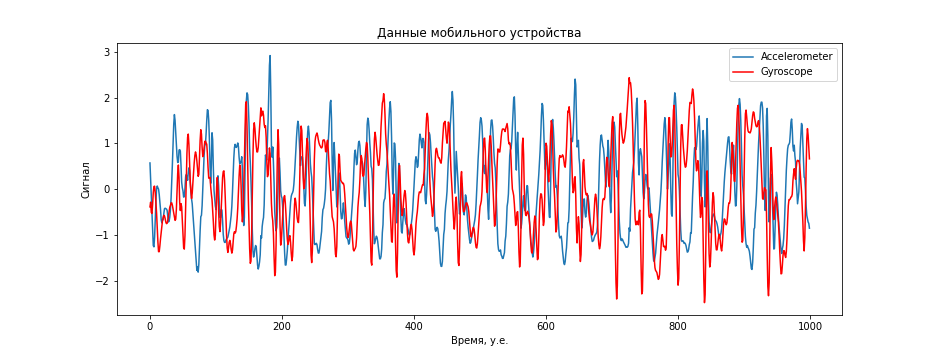
\includegraphics[width=1.1\textwidth]{./images/acc+gyr.png}}
\caption{Данные акселерометра и гироскопа одного мобильного устройтсва}
\label{fg:signal}
\end{figure}

\begin{figure}[h!]
\centering
  \subfloat[Акселерометр]{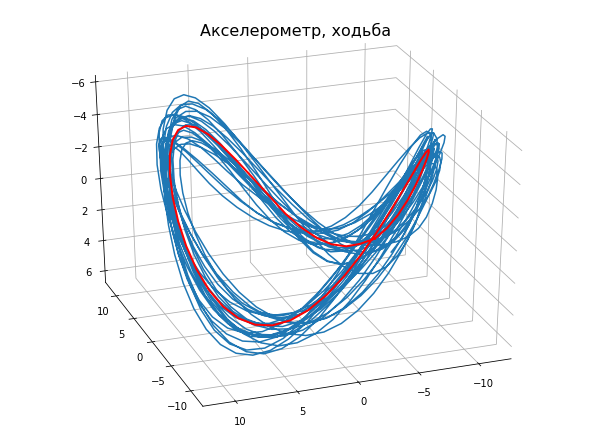
\includegraphics[width=0.6\textwidth]{./images/acc_tr_1.png}}
  \subfloat[Гироскоп]{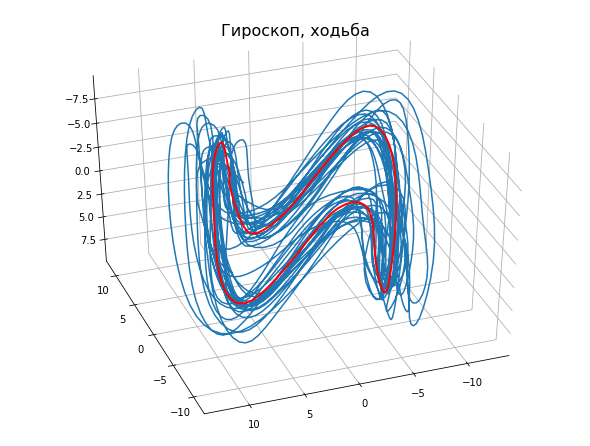
\includegraphics[width=0.6\textwidth]{./images/gyr_tr_1.png}}\\
\caption{Траектории в фазовом пространстве}
\label{fg:initial_traj}
\end{figure}


\begin{figure}[h!]
\centering
{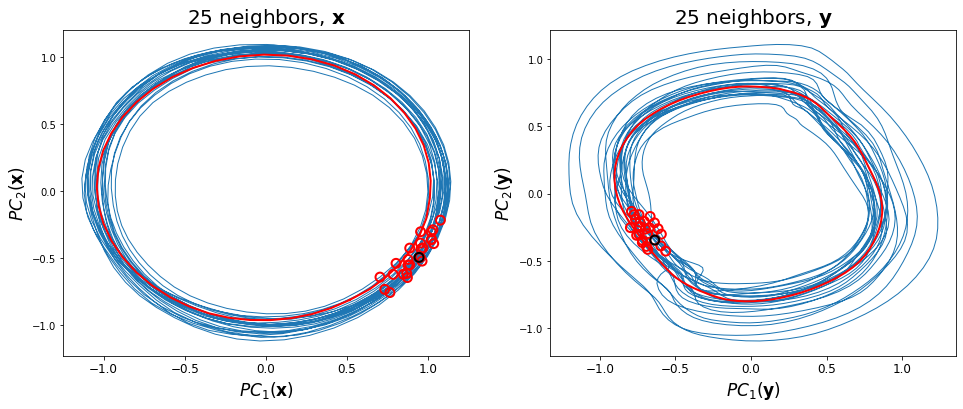
\includegraphics[width=1\textwidth]{./images/knn.png}}
\caption{Метод CCM для проверки наличия связи, PLS}
\label{fg:signal}
\end{figure}


\begin{figure}[h!]
\centering
{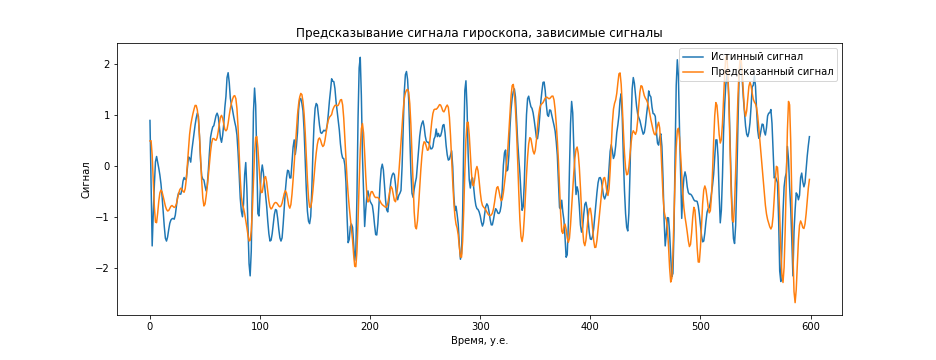
\includegraphics[width=1\textwidth]{./images/corr.png}}
\caption{Предсказание для зависимых сигналов, PLS}
\label{fg:signal}
\end{figure}

\begin{figure}[h!]
\centering
{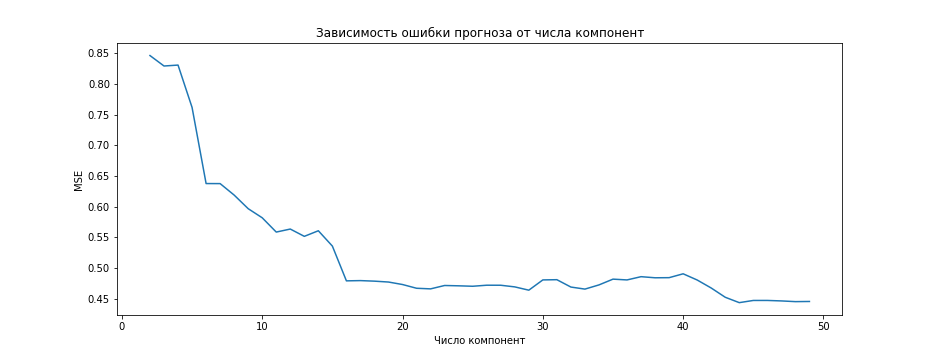
\includegraphics[width=1\textwidth]{./images/ERROR.png}}
\caption{Зависимость ошибки прогноза от числа компонент, зависимые ряды}
\label{fg:signal}
\end{figure}

Среднеквадратичная ошибка MSE = 0.48

\newpage 

\subsection{Несвязанные сигналы, aкселерометр + акселерометр}


\begin{figure}[h!]
\centering
{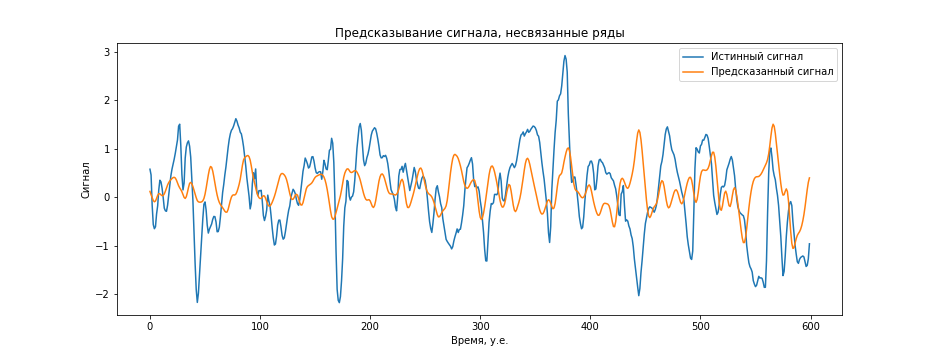
\includegraphics[width=1\textwidth]{./images/uncorr.png}}
\caption{Предсказание для несвязанных сигналов, PLS}
\label{fg:signal}
\end{figure}

\begin{figure}[h!]
\centering
{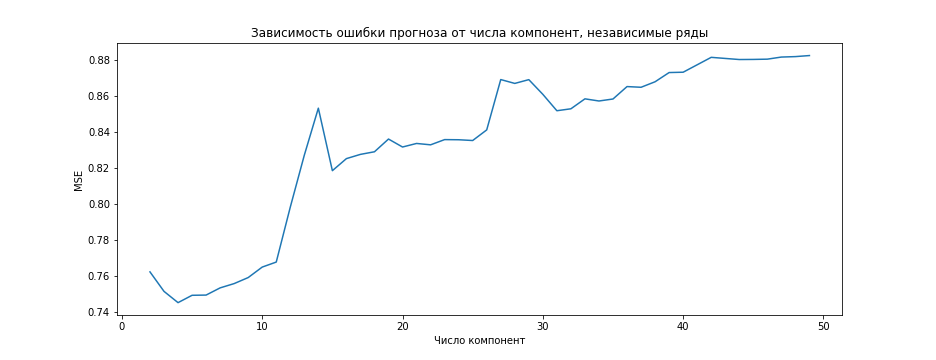
\includegraphics[width=1\textwidth]{./images/ERROR2.png}}
\caption{Зависимость ошибки прогноза от числа компонент, несвязанные ряды}
\label{fg:signal}
\end{figure}

Среднеквадратичная ошибка MSE = 0.86

\subsection{Медленная ходьба, акселерометр + гироскоп}

\begin{figure}[h!]
\centering
{\includegraphics[width=1.1\textwidth]{./images/signal_long.png}}
\caption{Данные акселерометра и гироскопа одного мобильного устройтсва}
\label{fg:signal}
\end{figure}

\begin{figure}[h!]
\centering
  \subfloat[Акселерометр]{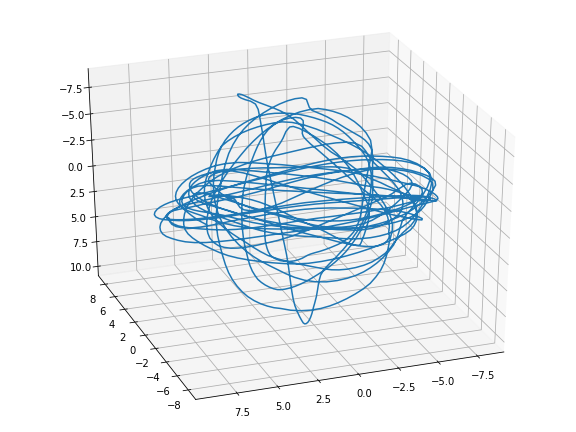
\includegraphics[width=0.6\textwidth]{./images/acc_tr_2.png}}
  \subfloat[Гироскоп]{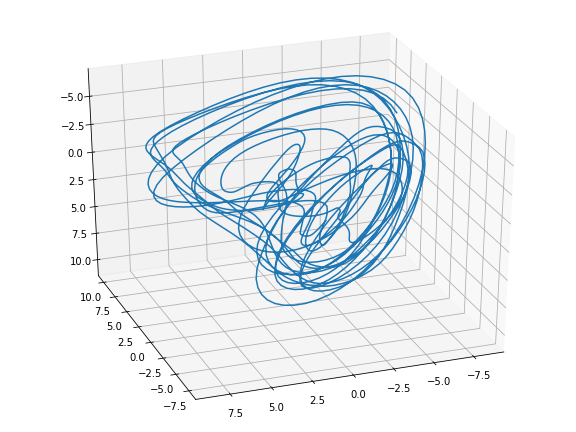
\includegraphics[width=0.6\textwidth]{./images/gyr_tr_2.png}}\\
\caption{Траектории в фазовом пространстве}
\label{fg:initial_traj}
\end{figure}

\begin{figure}[h!]
\centering
{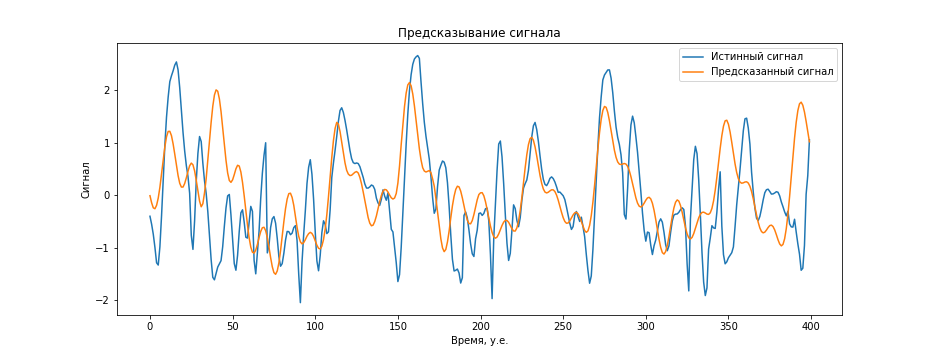
\includegraphics[width=1.1\textwidth]{./images/long_pls.png}}
\caption{Предсказание сигнала гироскопа, PLS}
\label{fg:signal}
\end{figure}

\newpage
% \section{Заключение}



% \bibliographystyle{unsrt}
% \bibliography{biblio}


\end{document}
